
\chapter{Fundamental Setup}
\label{sec:fepest:fundamentalSetup}

The fundamental setup prepares the model to be processed by PEST. Its steps are common to most PEST methods.

The fundamental setup comprises the definition of parameters, observations and prior knowledge (if available). A decision on using subspace methods is to be made, and finally, parallel computing may be configured to distribute workload on different computers.

\section{FEFLOW and FePEST}

FePEST requires a FEFLOW model as a starting point for any PEST setup. FePEST asks for the file name of the FEFLOW model when a new optimization project is created. 

When setting up a FEFLOW model that is planned to be subject to a PEST optimization, bear in mind that the run-times should be reasonably short and that the model must run stable.

It is possible to exchange the FEFLOW model by another one, provided that the new model file contains the same observation points and parameter zone selections (usually a modified version of the original model).

It is also possible to open a model simultaneously in FEFLOW and FePEST. If changes are made and the model is saved within FEFLOW, a reload must be performed within FePEST to inform it about the changes made.

\textit{Always perform a reload in FePEST after saving the FEM file in FEFLOW.}\marginpar{*}

\begin{figure}
	\center
	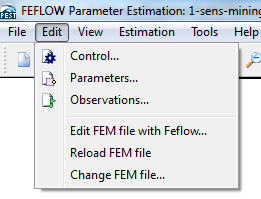
\includegraphics[width=0.7\columnwidth]{figureFundamentalSetup/FePESTEditMenu.png}
\caption{The Edit menu allows access to the problem settings dialog (Control / Parameters / Observations) and allows to open, reload and change the FEM file.}
\label{fig:fepest:FePESTEditMenu}
\end{figure} 

\section{Adjustable Parameters}

Choosing the model parameters that PEST can change to minimize the objective function is usually the first part of the setup.

An adjustable parameter can be described by its parameter type (e.g., hydraulic conductivity) and the zone of application (e.g., a certain geological formation).

\begin{itemize}
\item The \textbf{parameter type} can be any time-constant material property of the FEFLOW model. \marginpar{!}
\item The \textbf{zone} can be any elemental selection that is stored in the FEFLOW model.
\end{itemize}

Note that the choice for the zones already constitutes a kind of regularization (called structural regularization), that has the power to significantly influence the calibration process (in a good or bad way).

If making changes to elemental selections in FEFLOW, remember that you must reload the model after you have saved them in the FEFLOW file.
	
%See also \textit{Methodologies and Software for PEST-Based Model Predictive Uncertainty Analysis: Manual Regularization (p. 48) / Structural Regularization (p.50)}

%FePEST uses stored selections as zones; this step is done within the FEFLOW user interface. All sets of nodes or elements constituting zones in the PEST setup are selected and stored in the Spatial Units panel.
 	
\subsection{Definition of Parameters}

An optimization problem commonly comprises many parameters sharing identical or similar settings.

To avoid that the user needs to setup these parameters one-by-one, similar parameters are defined through a \textbf{parameter definition}. A parameter definition allows central adjustment of default values of its dependent parameters which are created from it. This allows convenient management of large lists of parameters.

Usage of a parameter definition differs depending on the choice of the assignment method. Possible assignment methods are:

\begin{itemize}
\item Zonally constant:

The user specifies one or multiple zones in which the value of a parameter is to be estimated. A dependent parameter will be created for each of these zones (see Figure \ref{fig:fepest:ParameterDefintionsZones}). During each model call of a PEST run, a constant value will be assigned to the chosen FEFLOW model property in each separate zone. 

\begin{figure}
	\center
	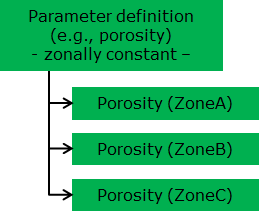
\includegraphics[width=0.7\columnwidth]{figureFundamentalSetup/ParameterDefintionsZones.png}
\caption{Zonal Parameter Definition}
\label{fig:fepest:ParameterDefintionsZones}
\end{figure}

\item Interpolate from pilot points:

The user chooses exactly one zone, which can be the model domain (a separate definition is required for each zone if pilot points are used). 

Within the limits of this zone, a cloud of pilot points is either imported from a file or is automatically generated by FePEST. Each of these points represents a single parameter of the PEST setup (see Figure \ref{fig:fepest:ParameterDefintionsPpoits})

\begin{figure}
	\center
	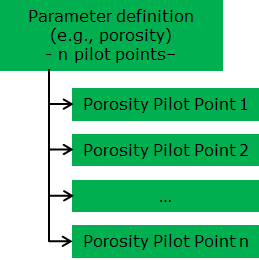
\includegraphics[width=0.7\columnwidth]{figureFundamentalSetup/ParameterDefintionsPpoits.png}
\caption{Pilot-Point Parameter Definition}
\label{fig:fepest:ParameterDefintionsPpoits}
\end{figure}

The parameter definition of a pilot-point based parameter includes the settings of the interpolation method that is used to interpolate parameter values between pilot points. Available options are Kriging and Radial Basis functions. 

Note that FePEST will apply the same settings to regularize the pilot-point parameters if the respective option for the Tikhonov Regularization is active.

\end{itemize}

The user can now define the settings that will be applied to the dependent parameters by default (individual changes can be done later). These include:

\begin{itemize}
	\item Transformation of the parameter
	\begin{itemize}
	\item logarithmic transformation often allows faster and quicker reduction of the objective function by linearization of the system)
	\item a parameter can be tied to a different parameter, in this case its value will be changed according to the parent parameter, always maintaining the ratio of their initial values
	\item a parameter can be fixed, thereby removing it from the optimization
\end{itemize}

\item Change limit

This setting defines how to determine the maximum offset with that a parameter can be changed within a single iteration. Note that relative change limits are not allowed if the parameter is log-transformed.

\item Initial value

The parameter value that is applied in the first iteration. The value assigned in the FEFLOW model will be used by default, assuming that this represents the preferred value of the expert modeller.

\item Bounds

An upper and a lower limit can be defined for the parameters. A good approach is to use a very low and very high value initially that does not impose a restriction to the optimization.

\item Scale and offset
Before a parameter value is assigned to the model run, it is multiplied with Scale and then added to Offset.

These settings usually do not need to be changed.
\end{itemize}

\begin{figure}
	\center
	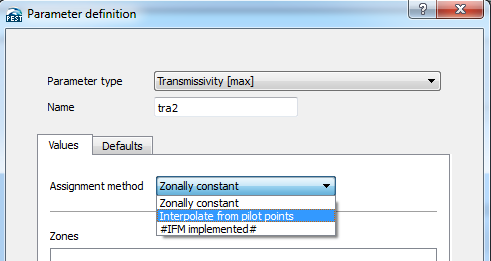
\includegraphics[width=\columnwidth]{figureFundamentalSetup/NewParameterDefinition.png}
\caption{Creating a new parameter definition. Choose from Zonally constant or pilot point interpolated parameter distributions. The Defaults tab defines the standard settings for the dependent parameters.}
\label{fig:fepest:NewParameterDefinition}
\end{figure}

\begin{figure}
	\center
	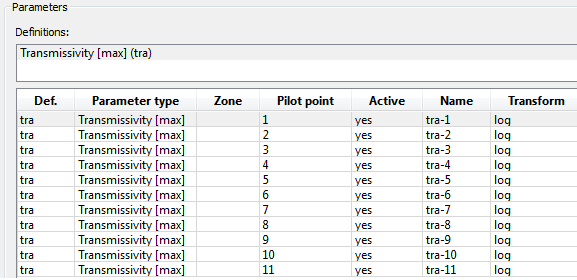
\includegraphics[width=\columnwidth]{figureFundamentalSetup/ParameterList.png}
\caption{After a parameter definition has been created (top), its dependent parameters appear in the list below.}
\label{fig:fepest:ParameterList}
\end{figure}

The OK button applies the new parameter definition. At the same time its dependent parameters are added to the parameter list.

These parameters inherit the default parameters of their parent definition. If required, changes to settings of individual parameters can be done (overriding the defaults), including the removal of parameters.

Working with large lists is easier with a spreadsheet program. The Copy/Paste buttons allow a quick transfer to and from other programs using the system clipboard.

Also see section \ref{sec:fepest:AdvancedMethods} for information on how to implement parameters through IFM plug-ins.

\subsection{Parameter Groups}
\label{sec:fepest:parameterGroupsSettings}

The parameter groups allows the configuration of the derivative calculation for the parameters (see section \ref{sec:fepest:derivativeCalculation}. FePEST applies default values that have been tested to work with most FEFLOW models, and often adjustments are not necessary when setting up a PEST model.

If the PEST optimization however fails due to bad derivatives calculations (which cannot be excluded as every model is different), a reconfiguration of these settings might be required. Detailed explanation and literature references to the different settings are given in the FePEST help system.

NOTE: The PEST utility tool JACTEST (section \ref{sec:fepest:Jactest}) is a utility to check for bad derivative calculation.

By default, FePEST defines one parameter group per FEFLOW parameter type and assigns the adjustable parameter to these groups accordingly:

\begin{itemize}
\item The Derivative method is chosen automatically (option "switch", starting with the more effective 2-point methods, switching to higher order methods if required)

\item The Increment size (set to 1.5\% by default) can be increased if minor model instability issues are observed. Do not increase this value unnecessary, as high values would violate the linearity assumption of the derivative calculation.
\end{itemize}

\section{Observations}

The observations provide the primary (and only) measure that informs the optimization algorithm about the model-to-measurement misfit.

For each observation FePEST requires:

\begin{itemize}
\item its type (e.g., hydraulic head),
\item its location (e.g. an observation data),
\item the time at that it was recorded (in case of a transient model) and
\item the value that was observed in reality.
\end{itemize}

Because the observation points set in FEFLOW already contains this information, it is possible to import them directly from the FEFLOW model.

By default, all observations are weighted with a weight of unity. These can be adapted by the user (compare section \ref{sec:fepest:observationWeights})

Supported observation types are all observations of system state (e.g., hydraulic head, saturation, mass concentration, temperature) depending on the models problem class. Reference values are constant values if the model is steady state. In a transient model, a time series contains the data of observations at different points in time.

Advanced users may also use IFM plug-ins or third party software for other types of observations.

%While the majority of observations will represent data that has actually been observed (in field or lab), there are some exceptions:

%\begin{itemize}
%\item Predictions (like an expected water table in the future) are futures observations of system state, and are often the actual purpose why the model has been built. Predictions are defined like usual (past observations), but with a weight of zero thus that the observation does not influence the objective funciton. It will however be visible in data plots and PEST will calculate the sensitivity to parameters.
%\item Planned observations can be investigated for its worthiness to reduce model uncertainty using advanced PEST functionality (not covered by this version of FePEST).
%\end{itemize}


\subsection{Definition of Observations}
\label{sec:fepest:observationDefintion}

Observations are defined in a similar way as parameters. If observations are of the same type (e.g., observations from the same well field), often similar or identical settings are required. 

For convenience, and to avoid many repetitive adaptations of these setting when creating or making changes to observations, each observation depends on an \textbf{observation definition}. A definition allows central adjustment of the default values of its dependent observations (see Figure \ref{fig:fepest:ObservationDefintion}. This allows a better management of a large number of observations.

\begin{figure}
	\center
	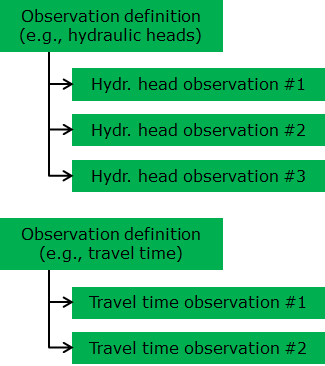
\includegraphics[width=0.7\columnwidth]{figureFundamentalSetup/ObservationDefinition.png}
\caption{Observation Definition}
\label{fig:fepest:ObservationDefinition}
\end{figure}

In the easiest case the definition of observations only requires the choice of the observation type (e.g., Hydraulic Head, Pressure, Mass concentration). 

\begin{itemize}
\item FePEST can automatically import the observation points of the given type from the FEFLOW model. If the model is transient, it adds multiple observations per observation point, each representing a sample point of the respective time series. A weight of one is applied by default.

\item Alternatively, an external file can provide the observation locations and data.

\item Advanced users may choose to create additional observations in the PEST setup, that can be implemented using IFM plug-ins or third-party software (see also section \ref{sec:fepest:AdvancedMethods}).

\end{itemize}

\begin{figure}
	\center
	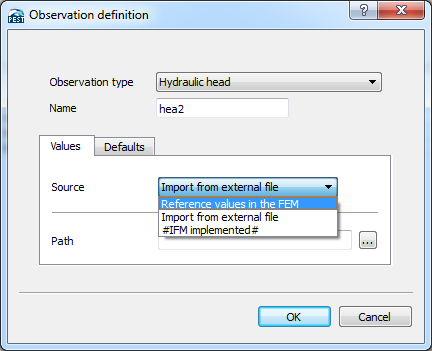
\includegraphics[width=\columnwidth]{figureFundamentalSetup/NewObservationDefinition.png}
\caption{Creating a new observation definition.}
\label{fig:fepest:NewObservationDefinition}
\end{figure}


Observations created in this way now populate the observation list (this being the actual list of observations as PEST sees it).

It is possible to change settings of particular observations (overriding the defaults). This is required especially when adapting the observation weights to achieve better optimization behavior and results.
 
HINT: Working with large lists is easier using a spreadsheet program. The Copy/Paste buttons allow a quick transfer to and from other programs using the system clipboard.

\subsection{Observation Groups}

FePEST automatically assigns observations of different type to different observation groups. This allows PEST to distinguish how much the different groups contribute to the measurement objective function.

In the same way it is possible to allocate observations of the same type to different groups (e.g., to differentiate between hydraulic head measurements in different aquifers). 

Advanced users may specify an observation covariance file to define the weights for these observations.

\section{Prior Knowledge}

Prior Knowledge - if available - can be described during this step of the PEST setup. In most cases the Tikhonov regularization option will be preferred over the manual setup of equations of prior information (see section \ref{sec:fepest:priorKnowledge} for details).

\subsection{Prior Information}

Equations of prior information allow to define preferred values for parameters, or preferred relations between parameters. Any deviation form this relationship will contribute to the regularization objective functions. As though there are certain similarities to observations:

\begin{itemize}

\item Name

A user-defined name to identify the equation.

\item Weight 

Each equation has a weight to allow to control the strength with that it contributes to the objective function (relative to other prior informations and field observations). Individual weights of prior information should reflect the trust that is associated with the underlying assumptions.

\item Group

It is possible to associate different prior informations to different observation groups, hereby defining more multiple regularization groups. The principle is the same as for the observation groups.

\end{itemize}

The formula itself has to be written in a special syntax specified in the PEST manual. Note that FePEST will not check for correct syntax on its own, however the PESTCHECK feature can performed from the Tools menu to do so (recommended after each change made to prior information).

A default formula is provided for convenience, which needs to be adapted for the specific purpose by the user.

\subsection{Tikhonov Regularization}

When activated, Tikhonov regularization can implement two different aspects of regularization in the PEST setup:

\begin{itemize}

\item Regularization based on initial parameter values

Assuming that the initial parameter value represent the expected values of the expert modeller, equations of prior information are created that will penalize departures of parameter values from initial values.

As a result, parameter values close to initial parameters will be preferred during the optimization.

\item Regularization of pilot point parameters using covariance matrices

Pilot-point type parameter values for each definition are regularized taking into account the expected correlation (using a covariance matrix). Differences in parameter values of pilot-points closer than their correlation length will be penalized.

As a result, homogeneous (smooth) parameter definitions will be preferred over heterogeneous ones.

\end{itemize}

\subsubsection{Objective Function Limits}

As it is described in section \ref{sec:fepest:priorKnowledge}, the Tikhonov regularization aims at finding a minimum of the regularization objective function, while maintaining user-defined limits for the measurement objective function (under which the model is still considered calibrated).

The following settings determine this limit:

\begin{itemize}

\item Target measurement objective function (PHIMLIM)

This is the limit for the measurement objective function below which the model is considered to be calibrated.

The value can be calculated by summing up the (weighted) measurement noise associated with the observations. If this is not possible, a value somewhat higher than the objective function that results from a calibration run without Tikhonov regularization can be chosen.

\item Acceptable measurement objective function (PHIMACCEPT)

This additional threshold is usually set slightly (5\% to 10\%) above PHIMLIM. PHIMLIM and PHIMACCEPT define a buffer zone for the measurement objective function value for stability reasons. In this zone, an objective function value is tolerated even though it does not meet the target value. This is necessary as the parameter upgrade vector will often "miss" the exact limit because it relies on a linearity assumption.

Figure \ref{fig:fepest:objectiveFunctionLimits} illustrates how the iteration adapts to these limits.

\begin{figure}
	\center
	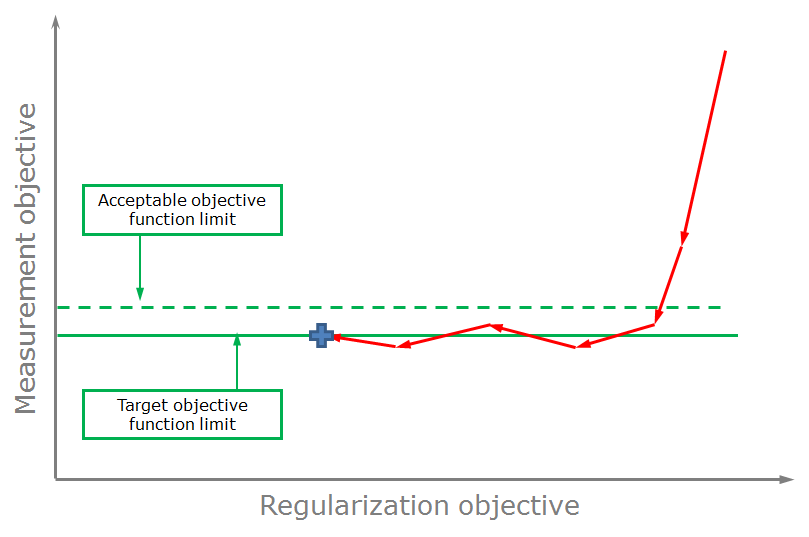
\includegraphics[width=\columnwidth]{figureFundamentalSetup/objectiveFunctionLimits.png}
\caption{Development of the regularization and measurement objective function during Tikhonov-regularized parameter estimation.}
\label{fig:fepest:objectiveFunctionLimits}
\end{figure}

\item Successive reduction of the objective function Limit (FRACPHIM)

This option allows a different strategy to determine the target objective function limits. If set to a non-zero value (allowed values are between 0 and 1), PHIMLIM is determined by multiplying the last achieved value of the measurement objective function with FRACPHIM.

In this way, PHIMLIM gets lower from iteration to iteration. It will however never be smaller than the value defined in PHIMLIM.

Optimal values for FRACPHIM are normally in the range 0.1 to 0.3. 

FePEST activates this option by default in combination with a very low objective function (these are the same defaults as applied by the PEST tool ADDREG1). This improves the well-posedness of the optimization and thereby leads to a more stable behavior of the GLMA optimization. The limits should however be adapted by the user as these settings might not yield the desired plausible parameter values. 

\end{itemize}

\textit{See Section 7.3.3 of the PEST user manual for a full discussion of these variables.}

\subsubsection{Weight Factors and Adjustment}

Settings to determine the weight factor can be used for fine tuning or trouble shootings. Their default values follow general recommendations that are suitable for most applications of PEST. 

\section{Subspace Regularization}

As described in section \ref{sec:fepest:SubSpaceReg} subspace regularization methods can greatly improve the stability and reduce the required modelling effort of an optimization.

\subsection{Singular Value Decomposition}

SVD is the recommended option for any PEST setup (unless LSQR has been chosen, which tends to be faster for PEST runs involving more than 2500 parameters). FePEST activates this option by default.

The particular settings determine how many singular values / super parameters are regarded during the optimization:

\begin{itemize}
\item The eigenvalue threshold, below which super parameters will be truncated, is by default set to 5e-7. At this value, the optimization is still regarded well-posed, which ensures stability of the optimization.

\item In addition, it is possible to further limit the number of singular values / super parameters to maximum number.
\end{itemize}

\textit{See the PEST users manual (5th Edition), section 8.4.2: Implementation of SVD with PEST for a full discussion of these settings.}

\subsection{SVD-Assist}

SVD-Assist (SVD-A) is useful to speed-up the calibration of highly parametrized models (often involving the pilot point method).

It can be chosen from two principle ways to determine the number of singular values:

\begin{itemize}

\item By default, PEST uses the SUPCALC tool to determine the optimal number automatically.

\item Manual specification of the number of super parameters can be useful if the run is carried out on multiple CPUs in parallel:

Each iteration requires one model run per super parameter to calculate the Jacobian matrix. Optimal usage of computational resources is given of the number of super parameters equals a multiple of total amounts of slaves (See section \ref{sec:fepest:parralelization}).
\end{itemize}

\section{Parallelization}
\label{sec:fepest:parralelization}

An inherent issue of calibration and uncertainty analysis, scenario runs and sensitivity analysis is the large number of required model calls and the often significant required run times.

Fortunately, many steps of a PEST run, especially the numerically expensive calculation of the Jacobian matrix, is very suitable for parallel computing. By involving a multitude of computers (whether this being a limited number of office PCs, a HPC cluster or cloud-based computers) computation times can be reduced to an acceptable level. But even if applied only locally on a single computer, parallelization can improve model run times significantly.

In case of highly-parametrized inversion processes, parallelization is often a requirement to finish a computation within typical project time frames.

FePEST deploys BeoPEST - a network capable version of PEST - for this task. FePEST also transfers the required model files to the slave computers. 

The port denotes the network (IP) port of the local computer (Host) that FePEST uses for communication. If the default settings conflicts with a different application, choose a different port number. Make sure that no router, firewall or anti-virus software blocks the network connection even if no remote computers are involved (localhost only).

Slaves shows the list of servers that will be used to undertake model run jobs during the PEST run (initially empty). You can add and remove servers to the list, or edit the settings of existing entries.

See also installation instructions for parallel computing.

\begin{itemize}
\item Host name

The host name specifies the host name or IP-address of the server computer. Enter "localhost" to add the local computer to the list.

Note that FePEST has to be started in server mode on all remote servers (except the local computer) before commencing the PEST run.

\item No. of Slaves

The number of slaves is the number of models that will be run simultaneously on the computer. In most cases, this will be set to the number of available CPU cores on that computer.

\end{itemize}

\begin{figure}
	\center
	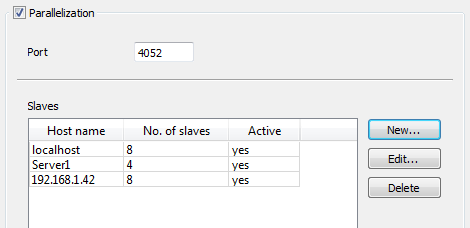
\includegraphics[width=\columnwidth]{figureFundamentalSetup/ParallelizationMenu.png}
\caption{The parallelization page contains the slave machines running FePEST in server mode.}
\label{fig:fepest:ParallelizationMenu}
\end{figure}

FePEST must be started and set to server mode (see Figure \ref{fig:fepest:StartServer}) on each of the slave servers.

\begin{figure}
	\center
	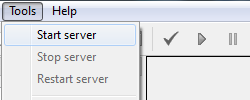
\includegraphics[width=0.7\columnwidth]{figureFundamentalSetup/StartServer.png}
\caption{When running in server mode, the current computer acts as a slave server that can receive run jobs from another computer.}
\label{fig:fepest:StartServer}
\end{figure}
